\chapter{Results}

This chapter presents the major results of this thesis. First, an optimal blending pattern for simultaneous crossline sources will be derived. Then, the advantages of a 3D $f$-$k_x$-$k_y$-filter towards a 2D $f$-$k$-filter will be shown. Finally, the feasibility of the suggested acquisition design will be proven on a synthetic 3D data set. 

 
\section{Blending pattern}


\begin{itemize}
	\item Explain how the acquisition limits the firing pattern
	\item Introduce spatial incoherency
	\item Suggest the applied blending pattern
	\item Show quality factor versus incoherency/firing pattern
\end{itemize}

An incoherent blending pattern is important for good deblending performance (see section \ref{sec:BlendingMatrix}). Different incoherent blending patterns will be tested, in particular, temporally and spatially incoherent blending patterns. 

This thesis considers the following blended acquisition set up: The sources are assembled in crossline direction and move in inline direction due to the vessel movement (see Figure \ref{fig:Ch-Theory-3D-BlendedAcquisition}). As a consequence each experiment can blend sources which belong to the same crossline. The source sampling rate in inline direction must be sufficiently small to avoid spatial aliasing. Thus, the sources within one crossline must be blended and recorded before the vessel reaches the next inline position.

Based on this set up there are three possibilities to blend the sources incoherently. First, the sources can be blended with random time delays (temporal incoherency). Second, one can randomly pick sources for each experiment (spatial incoherency). Third, temporal and spatial incoherency can be combined, i.e. randomly picked sources are blended with random time delays.

In the following these blending patterns will be tested on a synthetic data set. The deblending performance is evaluated with a quality factor, $Q$, according to \citet{IbrahimQuality}. The quality factor, $Q$, is defined as;

\begin{equation}
	Q = 10 \cdot \frac{\left|\left|\text{Unblended data}\right|\right| _2 ^2}{\left|\left|\text{Unblended data - Deblended data}\right|\right| _2 ^2} .	
\end{equation}
change

\begin{figure}
	\centering
	\begin{subfigure}[t]{0.8\textwidth}
		\centering
		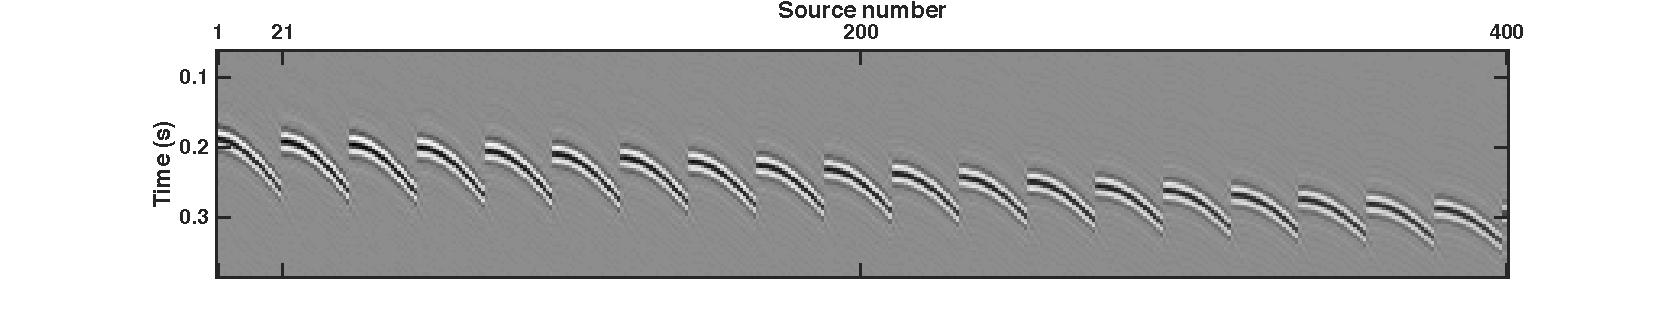
\includegraphics[width = \textwidth]{Plots/BlendingPatterns/Unblended_Delphi_zoom}
		\caption{}
		\label{fig:Ch-Results-Unbl-Delphi}
	\end{subfigure}
	%
	\centering
	\begin{subfigure}[t]{0.8\textwidth}
		\centering
		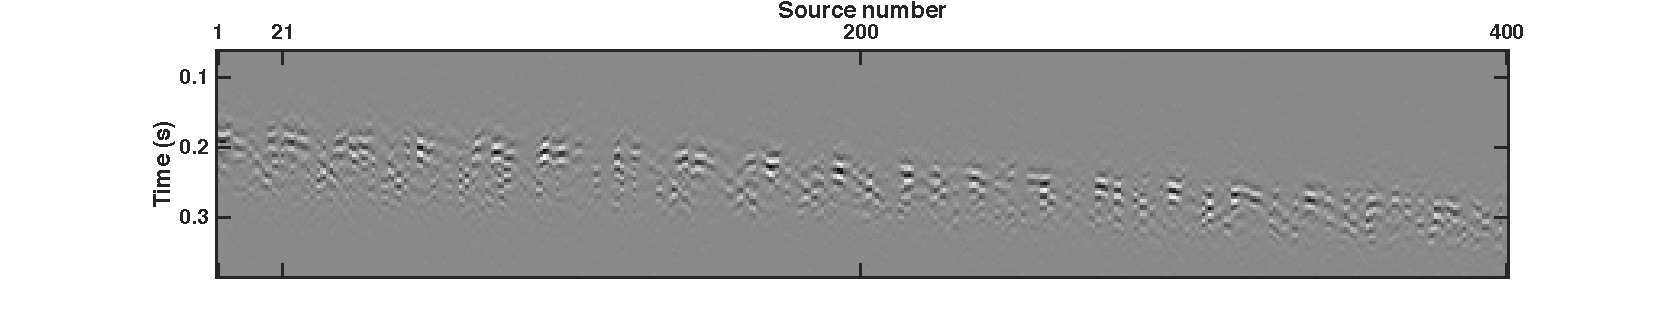
\includegraphics[width = \textwidth]{Plots/BlendingPatterns/Deblended_Delphi_zoomx}
		\caption{}
		\label{fig:Ch-Results-Debl-Delphi-x}
	\end{subfigure}
	%
	\centering
	\begin{subfigure}[t]{0.8\textwidth}
		\centering
		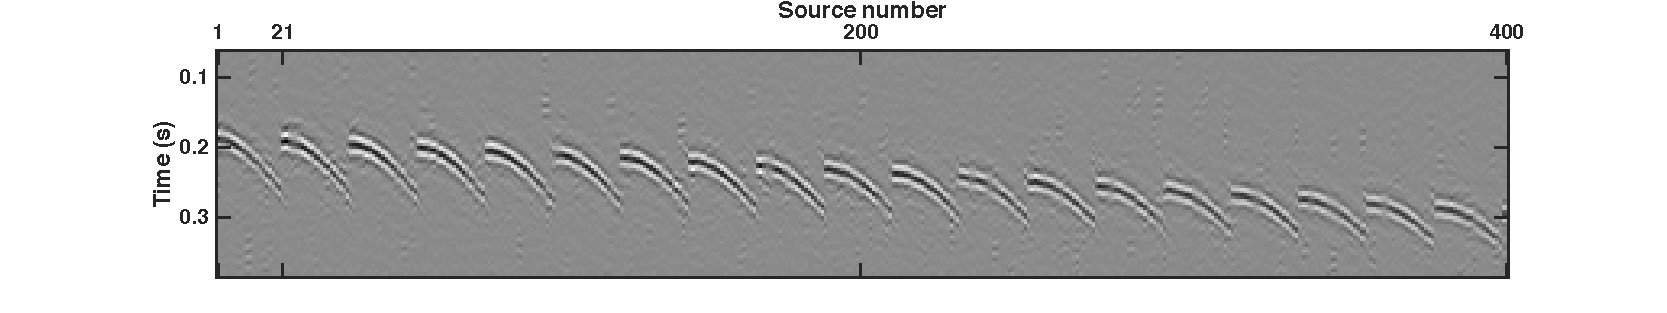
\includegraphics[width = \textwidth]{Plots/BlendingPatterns/Deblended_Delphi_zoomt}
		\caption{}
		\label{fig:Ch-Results-Debl-Delphi-t}
	\end{subfigure}
	%
	\centering
	\begin{subfigure}[t]{0.8\textwidth}
		\centering
		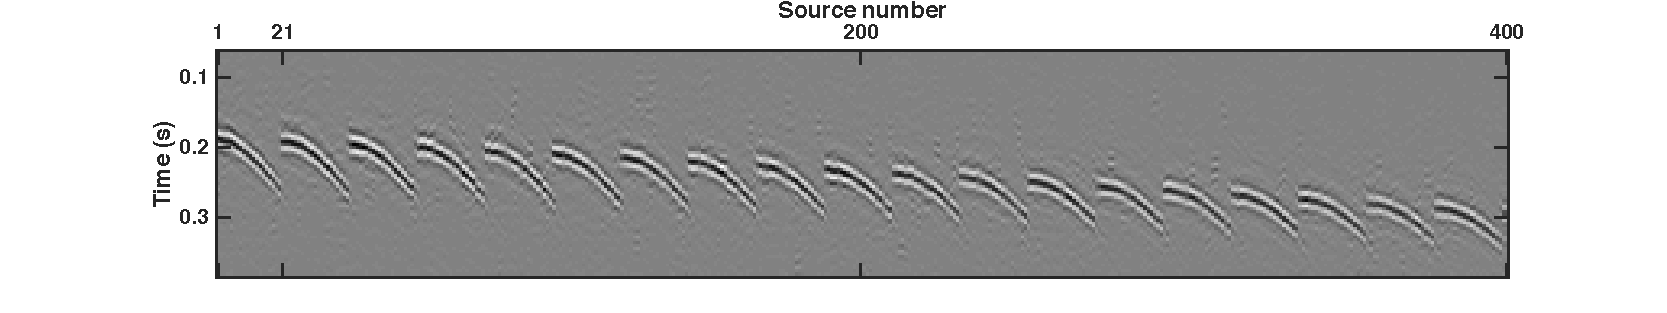
\includegraphics[width = \textwidth]{Plots/BlendingPatterns/Deblended_Delphi_zoomxt}
		\caption{}
		\label{fig:Ch-Results-Debl-Delphi-xt}
	\end{subfigure}
	%
\end{figure}

\section{3D FKK Filter Performance}

\section{Feasibility}








